\documentclass{article}
\usepackage{lmodern}
\usepackage[T1]{fontenc}
\usepackage[utf8]{inputenc}
\usepackage[pdftex]{graphicx}
\usepackage{amsmath}
\usepackage[spanish]{babel}
\usepackage{amsfonts}
\usepackage{amssymb}
\usepackage{amsmath,amssymb}
\addto\captionsspanish{
\def\listtablename{\'Indice de tablas}%
\def\tablename{Tabla}}
\usepackage{fancyhdr}
\usepackage{array}
\usepackage{wrapfig}
\usepackage{graphicx}
\usepackage[usenames]{color}
\usepackage{hyperref}
\usepackage{multicol}
\usepackage{enumitem}
\usepackage{multirow}
\usepackage{hyperref}
\usepackage{changepage}
\usepackage{float}
\usepackage[T1]{fontenc}
\usepackage{titlesec}
\usepackage{listings,lstautogobble}
\usepackage{tcolorbox}
\usepackage{booktabs} 
\usepackage{url}
\usepackage[export]{adjustbox}
\spanishdecimal{.}
\setlength{\parindent}{0cm}
\usepackage{amsmath}
\usepackage{pifont}
\usepackage[top=2.3cm,bottom=1.3in, left = 1.5cm , right = 1.5cm ]{geometry}
% bibliografia en ISO-690

\usepackage[backend=bibtex,
            style=iso-numeric,
            autocite=plain,
            maxbibnames=3,
            maxcitenames=1,
            urldate=long,
            uniquelist=false
]{biblatex}

\addbibresource{biblio.bib}

\hypersetup{
	colorlinks=true,
	linkcolor=black,
	filecolor=magenta,      
	urlcolor=cyan,
	pdftitle={Sharelatex Example},
}


%%%%%%%% COLOR ARDUINO

%%% Define Custom IDE Colors %%%
\definecolor{arduinoGreen}    {rgb} {0.17, 0.43, 0.01}
\definecolor{arduinoGrey}     {rgb} {0.47, 0.47, 0.33}
\definecolor{arduinoOrange}   {rgb} {0.8 , 0.4 , 0   }
\definecolor{arduinoBlue}     {rgb} {0.01, 0.61, 0.98}
\definecolor{arduinoDarkBlue} {rgb} {0.0 , 0.2 , 0.5 }

%%%%%% Arduino language
\lstdefinelanguage{Arduino}{
  language=C++, % begin with default C++ settings 
  %%% Keyword Color Group 1 %%%  (called KEYWORD3 by arduino)
  keywordstyle=\color{arduinoGreen},   
  deletekeywords={  % remove all arduino keywords that might be in c++
                break, case, override, final, continue, default, do, else, for, 
                if, return, goto, switch, throw, try, while, setup, loop, export, 
                not, or, and, xor, include, define, elif, else, error, if, ifdef, 
                ifndef, pragma, warning,
                HIGH, LOW, INPUT, INPUT_PULLUP, OUTPUT, DEC, BIN, HEX, OCT, PI, 
                HALF_PI, TWO_PI, LSBFIRST, MSBFIRST, CHANGE, FALLING, RISING, 
                DEFAULT, EXTERNAL, INTERNAL, INTERNAL1V1, INTERNAL2V56, LED_BUILTIN, 
                LED_BUILTIN_RX, LED_BUILTIN_TX, DIGITAL_MESSAGE, FIRMATA_STRING, 
                ANALOG_MESSAGE, REPORT_DIGITAL, REPORT_ANALOG, SET_PIN_MODE, 
                SYSTEM_RESET, SYSEX_START, auto, int8_t, int16_t, int32_t, int64_t, 
                uint8_t, uint16_t, uint32_t, uint64_t, char16_t, char32_t, operator, 
                enum, delete, bool, boolean, byte, char, const, false, float, double, 
                null, NULL, int, long, new, private, protected, public, short, 
                signed, static, volatile, String, void, true, unsigned, word, array, 
                sizeof, dynamic_cast, typedef, const_cast, struct, static_cast, union, 
                friend, extern, class, reinterpret_cast, register, explicit, inline, 
                _Bool, complex, _Complex, _Imaginary, atomic_bool, atomic_char, 
                atomic_schar, atomic_uchar, atomic_short, atomic_ushort, atomic_int, 
                atomic_uint, atomic_long, atomic_ulong, atomic_llong, atomic_ullong, 
                virtual, PROGMEM,
                Serial, Serial1, Serial2, Serial3, SerialUSB, Keyboard, Mouse,
                abs, acos, asin, atan, atan2, ceil, constrain, cos, degrees, exp, 
                floor, log, map, max, min, radians, random, randomSeed, round, sin, 
                sq, sqrt, tan, pow, bitRead, bitWrite, bitSet, bitClear, bit, 
                highByte, lowByte, analogReference, analogRead, 
                analogReadResolution, analogWrite, analogWriteResolution, 
                attachInterrupt, detachInterrupt, digitalPinToInterrupt, delay, 
                delayMicroseconds, digitalWrite, digitalRead, interrupts, millis, 
                micros, noInterrupts, noTone, pinMode, pulseIn, pulseInLong, shiftIn, 
                shiftOut, tone, yield, Stream, begin, end, peek, read, print, 
                println, available, availableForWrite, flush, setTimeout, find, 
                findUntil, parseInt, parseFloat, readBytes, readBytesUntil, readString, 
                readStringUntil, trim, toUpperCase, toLowerCase, charAt, compareTo, 
                concat, endsWith, startsWith, equals, equalsIgnoreCase, getBytes, 
                indexOf, lastIndexOf, length, replace, setCharAt, substring, 
                toCharArray, toInt, press, release, releaseAll, accept, click, move, 
                isPressed, isAlphaNumeric, isAlpha, isAscii, isWhitespace, isControl, 
                isDigit, isGraph, isLowerCase, isPrintable, isPunct, isSpace, 
                isUpperCase, isHexadecimalDigit, 
                }, 
  morekeywords={   % add arduino structures to group 1
                break, case, override, final, continue, default, do, else, for, 
                if, return, goto, switch, throw, try, while, setup, loop, export, 
                not, or, and, xor, include, define, elif, else, error, if, ifdef, 
                ifndef, pragma, warning,
                }, 
% 
%
  %%% Keyword Color Group 2 %%%  (called LITERAL1 by arduino)
  keywordstyle=[2]\color{arduinoBlue},   
  keywords=[2]{   % add variables and dataTypes as 2nd group  
                HIGH, LOW, INPUT, INPUT_PULLUP, OUTPUT, DEC, BIN, HEX, OCT, PI, 
                HALF_PI, TWO_PI, LSBFIRST, MSBFIRST, CHANGE, FALLING, RISING, 
                DEFAULT, EXTERNAL, INTERNAL, INTERNAL1V1, INTERNAL2V56, LED_BUILTIN, 
                LED_BUILTIN_RX, LED_BUILTIN_TX, DIGITAL_MESSAGE, FIRMATA_STRING, 
                ANALOG_MESSAGE, REPORT_DIGITAL, REPORT_ANALOG, SET_PIN_MODE, 
                SYSTEM_RESET, SYSEX_START, auto, int8_t, int16_t, int32_t, int64_t, 
                uint8_t, uint16_t, uint32_t, uint64_t, char16_t, char32_t, operator, 
                enum, delete, bool, boolean, byte, char, const, false, float, double, 
                null, NULL, int, long, new, private, protected, public, short, 
                signed, static, volatile, String, void, true, unsigned, word, array, 
                sizeof, dynamic_cast, typedef, const_cast, struct, static_cast, union, 
                friend, extern, class, reinterpret_cast, register, explicit, inline, 
                _Bool, complex, _Complex, _Imaginary, atomic_bool, atomic_char, 
                atomic_schar, atomic_uchar, atomic_short, atomic_ushort, atomic_int, 
                atomic_uint, atomic_long, atomic_ulong, atomic_llong, atomic_ullong, 
                virtual, PROGMEM,
                },  
% 
%
  %%% Keyword Color Group 3 %%%  (called KEYWORD1 by arduino)
  keywordstyle=[3]\bfseries\color{arduinoOrange},
  keywords=[3]{  % add built-in functions as a 3rd group
                Serial, Serial1, Serial2, Serial3, SerialUSB, Keyboard, Mouse,
                },      
%
%
  %%% Keyword Color Group 4 %%%  (called KEYWORD2 by arduino)
  keywordstyle=[4]\color{arduinoOrange},
  keywords=[4]{  % add more built-in functions as a 4th group
                abs, acos, asin, atan, atan2, ceil, constrain, cos, degrees, exp, 
                floor, log, map, max, min, radians, random, randomSeed, round, sin, 
                sq, sqrt, tan, pow, bitRead, bitWrite, bitSet, bitClear, bit, 
                highByte, lowByte, analogReference, analogRead, 
                analogReadResolution, analogWrite, analogWriteResolution, 
                attachInterrupt, detachInterrupt, digitalPinToInterrupt, delay, 
                delayMicroseconds, digitalWrite, digitalRead, interrupts, millis, 
                micros, noInterrupts, noTone, pinMode, pulseIn, pulseInLong, shiftIn, 
                shiftOut, tone, yield, Stream, begin, end, peek, read, print, 
                println, available, availableForWrite, flush, setTimeout, find, 
                findUntil, parseInt, parseFloat, readBytes, readBytesUntil, readString, 
                readStringUntil, trim, toUpperCase, toLowerCase, charAt, compareTo, 
                concat, endsWith, startsWith, equals, equalsIgnoreCase, getBytes, 
                indexOf, lastIndexOf, length, replace, setCharAt, substring, 
                toCharArray, toInt, press, release, releaseAll, accept, click, move, 
                isPressed, isAlphaNumeric, isAlpha, isAscii, isWhitespace, isControl, 
                isDigit, isGraph, isLowerCase, isPrintable, isPunct, isSpace, 
                isUpperCase, isHexadecimalDigit, 
                },      
%
%
  %%% Set Other Colors %%%
  stringstyle=\color{arduinoDarkBlue},    
  commentstyle=\color{arduinoGrey},    
%          
%   
  %%%% Line Numbering %%%%
   numbers=left,                    
  numbersep=5pt,                   
  numberstyle=\color{arduinoGrey},    
  %stepnumber=2,                      % show every 2 line numbers
%
%
  %%%% Code Box Style %%%%
  breaklines=true,                    % wordwrapping
  tabsize=2,         
  basicstyle=\ttfamily  
}
%%%%%%%%%%%%%%%%%%%%%%%%%%%%%%%%%%%%%%%%%
\definecolor{bodyexample}{RGB}{191, 223, 223}
\definecolor{titleexample}{RGB}{0, 127, 127}
\definecolor{colorusach}{RGB}{24, 164, 153}
\definecolor{colorusachbody}{RGB}{226, 244, 242}
\definecolor{alerblockcolortitle}{RGB}{235, 119, 4}
\definecolor{alerblockcolorbody}{RGB}{255, 223, 191}

\newtcolorbox{bodyblock}[3][]
{
  colframe = colorusach!25,
  colback  = colorusachbody!10,
  coltitle = black!20!black,  
  title    = {#3},
  #1,
}


\newtcolorbox{alerblock}[3][]
{
  colframe = red!25,
  colback  = colorusachbody!10,
  coltitle = black!20!black,  
  title    = {#3},
  #1,
}

\renewcommand\theequation{\alph{equation}}


\fancypagestyle{sinfooter}{      
  \lhead{%
  \begin{minipage}[t]{0.3\textwidth} % Alinea el logo a la izquierda
    
\includegraphics[width=\linewidth]{images/DIMECLOGO.png}
  \end{minipage}
  }

  \rhead{%
  \begin{minipage}[b]{0.6\textwidth} % Alinea el texto a la derecha
  \raggedleft % Alinea el texto a la derecha
  \textsc{Universidad de Santiago de Chile \\
  Facultad de Ingeniería \\
  Open Robotics}
  \end{minipage}

  }
  % Configura la línea horizontal en el encabezado
  \renewcommand{\headrulewidth}{0.4pt}
  \cfoot{}
}




\pagestyle{fancy}

% Configura el encabezado (izquierda, centro, derecha)
\lhead{%
  \begin{minipage}[t]{0.3\textwidth} % Alinea el logo a la izquierda
    
\includegraphics[width=\linewidth]{images/DIMECLOGO.png}
  \end{minipage}
}

\rhead{%
\begin{minipage}[b]{0.6\textwidth} % Alinea el texto a la derecha
  \raggedleft % Alinea el texto a la derecha
  \textsc{Universidad de Santiago de Chile \\
  Facultad de Ingeniería \\
  Open Robotics}
\end{minipage}

}
% Configura la línea horizontal en el encabezado
\renewcommand{\headrulewidth}{0.4pt}
% Configura el pie de página
\cfoot{\thepage} % Coloca el número de página en el centro del pie de página


\setlength{\headsep}{75pt}

\begin{document}

\numberwithin{equation}{section}

\vspace*{5cm}
\begin{center}
  \LARGE{Tutorial Aplicación ROS}\\
  \large{Control de turtlesim con Joystick Arduino}\\
  \vspace*{1cm}
  \large{Autor: René Torres}\\
  \large{Fecha: \today}
\end{center}


\thispagestyle{sinfooter} % Aplica el estilo para borrar el número en la primera página de portada

\newpage

\tableofcontents

\newpage


\section{Introducción}

En este documento se detalla el proceso de instalación y configuración de un proyecto de ROS, el cual consiste en el control de la tortuga de turtlesim mediante un joystick conectado a un arduino. El proyecto se encuentra disponible en el repositorio de github: \url{https://github.com/ReneTorresA/jstk_turtlesim}.\\

La aplicación esta configurada para que al presionar el botón del joystick se mueva la tortuga de forma aleatoria en el espacio de trabajo de turtlesim, como se muestra en la figura \ref{fig:turtlesim}, y además se cambie el color y espesor del trayecto de la tortuga de forma aleatoria.

\begin{figure}[H]
  \centering
  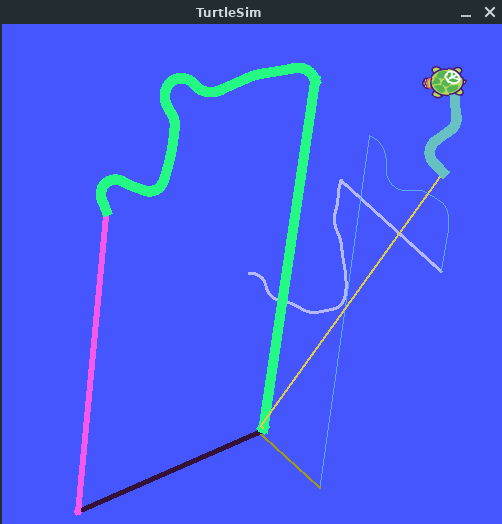
\includegraphics[width=0.6\textwidth ]{images/turtlesim.png}
  \caption{Espacio de trabajo de turtlesim.}
  \label{fig:turtlesim}
\end{figure}



\section{Instalación de Dependencias}

Para que este proyecto funcione adecuadamente es necesario instalar las siguientes dependencias y software:

\begin{enumerate}
  \item ROS Noetic: \url{http://wiki.ros.org/noetic}
  \item Libreria Rosserial Arduino: \url{http://wiki.ros.org/rosserial_arduino/Tutorials/Arduino%20IDE%20Setup}
  \item Arduino IDE: \url{https://www.arduino.cc/en/software}
  \item Python 3: \url{https://www.python.org/}
\end{enumerate}

El sistema operativo usado en este proyecto es una distribución de Linux basada en \textbf{Ubuntu 20.04}.





\subsection{Diagrama de conexión y configuración de arduino}


Para este proyecto es necesario contar con una placa de arduino y un modulo de joystick, a continuación en la figura \ref{fig:diagrama} se muestra el diagrama de conexión de los componentes.


\begin{figure}[H]
  \centering
  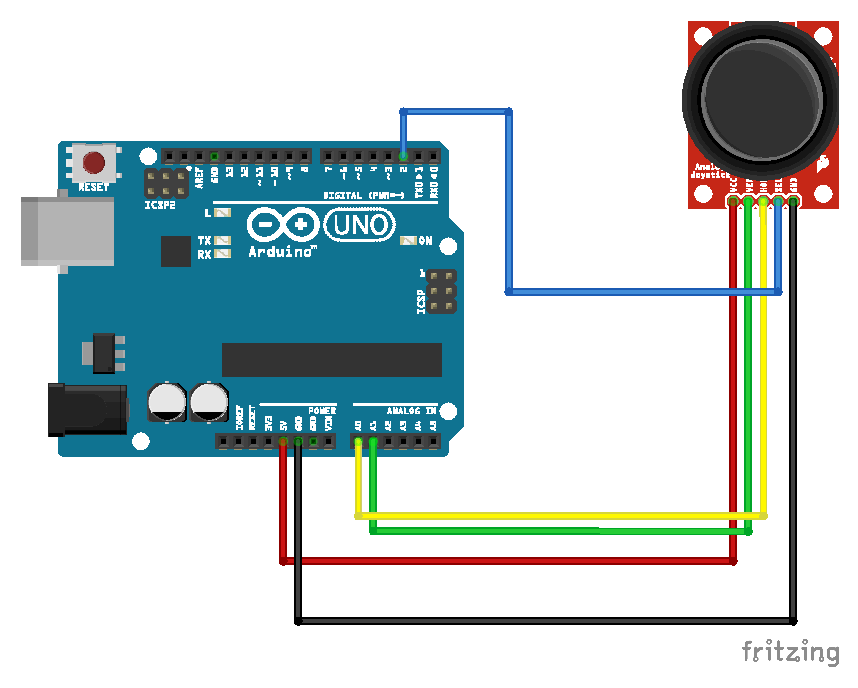
\includegraphics[width=0.7\textwidth]{images/diagrama_conexiones.pdf}
  \caption{Diagrama de conexión.}
  \label{fig:diagrama}
\end{figure}

Una vez realizada las conexiones se procede a modificar (si es necesario) y cargar el código de arduino en la placa, el cual se encuentra en el repositorio de github y adjunto en el apéndice, sección \ref{sec:codigo_arduino}. Se recomienda que verifique que su placa de arduino este conectada correctamente y que guarde el nombre del puerto serial, ya que lo necesitara para modificar el archivo .

Para saber que puerto está usando su placa de arduino puede visualizarlo en la aplicación de Arduino IDE, como se muestra en la figura \ref{fig:puerto}.

\begin{figure}[H]
  \centering
  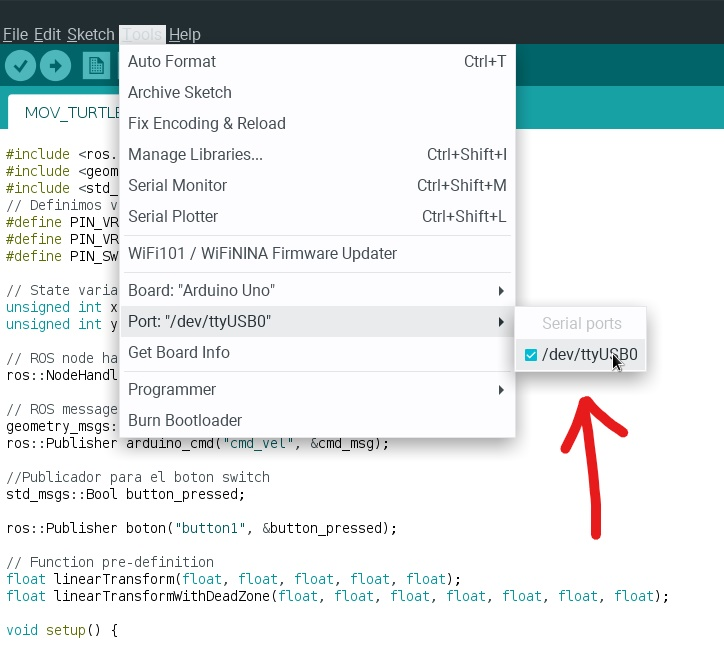
\includegraphics[width=0.7\textwidth]{images/usbarduino.jpg}
  \caption{Puerto serial de arduino.}
  \label{fig:puerto}
\end{figure}

En este caso el puerto serial es \textbf{/dev/ttyUSB0}, por lo que hay que asegurar que en el archivo \textbf{jstk\_turtlesim.launch} que se encuentra en la carpeta \textbf{launch} de la aplicación, en la etiqueta con nombre "port" en el apartado default tiene que estar el nombre correcto del puerto, como se muestra a continuación:

\begin{verbatim} jstk\_turtlesim.launch

  <launch>
    <!-- Start turtlesim_node node -->
    <node name="turtlesim" pkg="turtlesim" type="turtlesim_node"/>
  
    <!-- Start rqt_graph for node visualization -->
    <node name="rqt_graph" pkg="rqt_graph" type="rqt_graph"/>
  
    <!-- Start button_suscriber node for call service -->
    <node name="listener_button" pkg="jstk_turtlesim" type="button_suscriber.py"/>
  
    <!-- Rosserial arduino node -->
    <arg name="port" default="/dev/ttyUSB0"/>
  
    <node name="arduino_node" pkg="rosserial_python" type="serial_node.py">
      <param name="port" type="string" value="$(arg port)"/>
      <remap from="cmd_vel" to="turtle1/cmd_vel"/>
    </node>
  </launch>
\end{verbatim}

\section{Uso de la aplicación}

Para usar la aplicación se recomienda seguir los siguientes pasos:\\

\textbf{Paso 1:} Clone el repositorio de github en la carpeta \textbf{src} de su espacio de trabajo de ROS. Para esto abra una terminal y ejecute el siguiente comando:

\begin{bodyblock}{red}{ \textbf{Paso 1}}
  \begin{lstlisting}[language=bash, mathescape=true, breaklines=true,numbers=left,
    xleftmargin=0.03\textwidth, columns=fullflexible, flexiblecolumns=true, gobble=8]
        cd ~/catkin_ws/src
        git clone https://github.com/ReneTorresA/jstk_turtlesim.git
  \end{lstlisting}
\end{bodyblock}

\subsection{Estructura del proyecto}

La estructura, luego de ser clonado el respositorio, deberia quedar de la siguiente forma:

\begin{center}
  \begin{verbatim}
    catkin_ws
    |-- CMakeLists.txt
    |-- package.xml
    |-- build
    |-- devel
    |-- src
        |-- jstk_turtlesim
            |-- src
                |-- scripts
                    |-- button_subscriber.py
                |-- launch
                    |-- jstk_turtlesim.launch
                |-- arduino
                    |-- jstk_turtlesim.ino
                |-- docs
                    |-- presentacion
                        |-- presentacion.pdf
                        |-- presentacion_latex
                    |-- tutorial
                        |-- tutorial.pdf
                        |-- tutorial_latex
                |-- CMakeLists.txt
                |-- package.xml
  \end{verbatim}
  
\end{center}

Una vez clonado el repositorio se recomienda agregar el \textit{path} a la terminal. Para esto ejecute el siguiente comando en la carpta del espacio de trabajo:

\begin{bodyblock}{red}{ \textbf{Paso 2}}
  \begin{lstlisting}[language=bash, mathescape=true, breaklines=true,numbers=left,
    xleftmargin=0.03\textwidth, columns=fullflexible, flexiblecolumns=true, gobble=8]
        cd ~/catkin_ws
        source devel/setup.bash 
  \end{lstlisting}
\end{bodyblock}

\textbf{Paso 3:} Para ejecutar la aplicación ejecute el siguiente comando en la terminal:

\begin{bodyblock}{red}{ \textbf{Paso 3}}
  \begin{lstlisting}[language=bash, mathescape=true, breaklines=true,numbers=left,
    xleftmargin=0.03\textwidth, columns=fullflexible, flexiblecolumns=true, gobble=8]
        roslaunch jstk_turtlesim jstk_turtlesim.launch
  \end{lstlisting}
\end{bodyblock}

Si todo ha salido bien debería ver la aplicación de turtlesim y el nodo de rqt\_graph, como se muestra en las figuras \ref{fig:turtlesim2} y \ref{fig:joystick}, respectivamente. Si presiona el botón del joystick debería ver que la tortuga se mueve de forma aleatoria en el espacio de trabajo de turtlesim y que el color y espesor del trayecto de la tortuga cambia de forma aleatoria, con el joystick puede controlar el movimiento de la tortuga lineal y angularmente.

\begin{figure}[H]
  \centering
  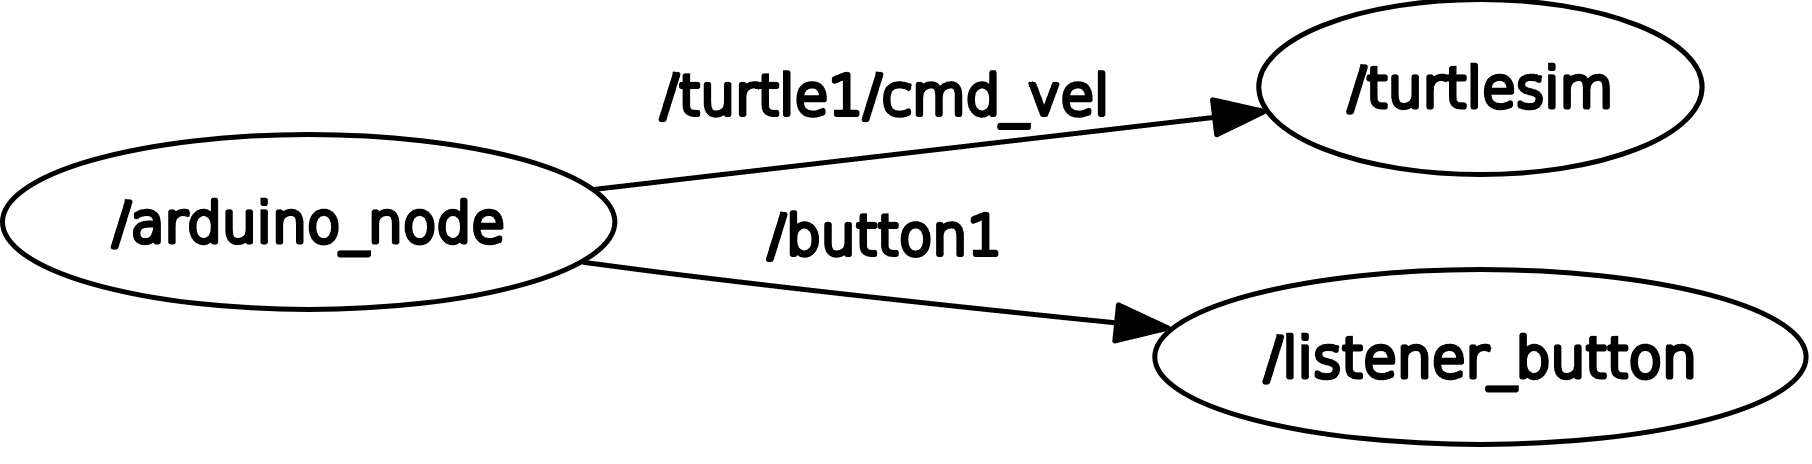
\includegraphics[width=0.7\textwidth]{images/rqtgraph.png}
  \caption{Comunicación entre nodos.}
  \label{fig:joystick}
\end{figure}

\begin{figure}[H]
  \centering
  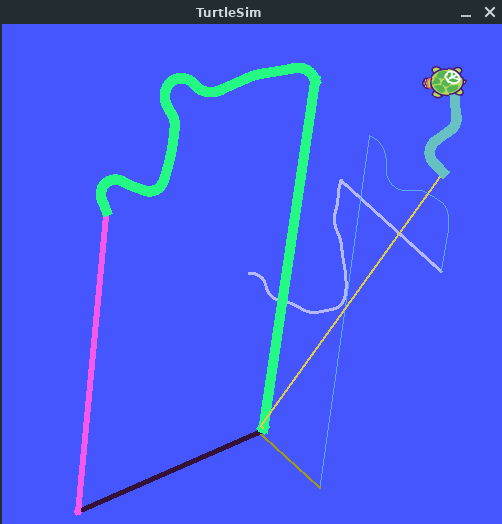
\includegraphics[width=0.45\textwidth ]{images/turtlesim.png}
  \caption{Espacio de trabajo de turtlesim.}
  \label{fig:turtlesim2}
\end{figure}




\newpage

\lstdefinestyle{mystyle}{
      backgroundcolor=\color{white},    % Fondo blanco
      basicstyle=\color{black},         % Texto en color negro
      keywordstyle=\color{blue},        % Palabras clave en azul
      commentstyle=\color{green},       % Comentarios en verde
  }
  

\nocite{clase,ros}


\printbibliography[heading=bibintoc,title={Referencias}]


\newpage
\section{Apéndice}
\subsection{Nodo button\_suscriber.py}
\begin{bodyblock}{red}{ \textbf{button\_suscriber.py}}
  \begin{lstlisting}[language=Python, mathescape=true, breaklines=true,numbers=left,
    xleftmargin=0.03\textwidth, columns=fullflexible, flexiblecolumns=true, gobble=8,style=mystyle]    
        #!/usr/bin/env python3

        import rospy
        from std_msgs.msg import Bool
        import random
        from turtlesim.srv import TeleportAbsolute, TeleportAbsoluteRequest, SetPen,SetPenRequest
        # Function when a message is received
        def callback(data):
          rospy.wait_for_service('/turtle1/teleport_absolute')
          spawn_client = rospy.ServiceProxy('/turtle1/teleport_absolute',TeleportAbsolute)

          request = TeleportAbsoluteRequest()

          request.x = random.uniform(0,11)
          request.y = random.uniform(0,11)
          request.theta = random.uniform(0,3.1416)

          rospy.wait_for_service('/turtle1/set_pen')
          set_pen_client = rospy.ServiceProxy('/turtle1/set_pen',SetPen)
          requestdos=SetPenRequest()
          requestdos.r = random.randint(0,255) 
          requestdos.g = random.randint(0,255)
          requestdos.b = random.randint(0,255)
          requestdos.width = random.randint(0,10)
              
        if data.data == True:
          spawn_client(request)
          set_pen_client(requestdos)
          rospy.loginfo("La tortuga ha sido movida aleatoriamente")
        else:
          rospy.loginfo(f"Esperando por el servicio")

        rospy.init_node('listener_ button') # Create node
        rospy.Subscriber('/button1', Bool, callback)   # Create subscriber
        rospy.spin()                # Wait for a message
\end{lstlisting}
\end{bodyblock}


\subsection{Código Arduino (\textbf{jstk\_turtlesim.ino})}{\label{sec:codigo_arduino}}


\begin{bodyblock}{red}{ \textbf{jstk\_turtlesim.ino}}

  \begin{lstlisting}[language=Arduino, mathescape=true, breaklines=true,numbers=left,
    xleftmargin=0.03\textwidth, columns=fullflexible, flexiblecolumns=true, gobble=8]
        // Incluimos las librerias necesarias de ROS
        #include <ros.h>
        #include <geometry_msgs/Twist.h>
        #include <std_msgs/Bool.h>
        // Definimos variables para los puertos del Arduino
        #define PIN_VRx A0
        #define PIN_VRy A1
        #define PIN_SW 2

        // State variables
        unsigned int xJoystick = 0;
        unsigned int yJoystick = 0;
        // ROS node handle
        ros::NodeHandle nh;
        // ROS message and publisher
        geometry_msgs::Twist cmd_msg;
        ros::Publisher arduino_cmd("cmd_vel", &cmd_msg);
        //Publicador para el boton switch
        std_msgs::Bool button_pressed;
        ros::Publisher boton("button1", &button_pressed);
        // Function pre-definition
        float linearTransform(float, float, float, float, float);
        float linearTransformWithDeadZone(float, float, float, float, float, float, float);
        void setup() {
        pinMode(PIN_SW,INPUT_PULLUP);
        nh.initNode();
        nh.advertise(arduino_cmd);
        nh.advertise(boton);
        while(!nh.connected()) {
          nh.spinOnce();
        }
        nh.loginfo("Startup complete!");
        }
\end{lstlisting}
\end{bodyblock}


\begin{bodyblock}{red}{ \textbf{jstk\_turtlesim.ino}}

  \begin{lstlisting}[language=Arduino,firstnumber=44, mathescape=true, breaklines=true,numbers=left,
    xleftmargin=0.03\textwidth, columns=fullflexible, flexiblecolumns=true, gobble=8]
        void loop() {

        // Read data from joystick
        xJoystick = analogRead(PIN_VRx);
        yJoystick = analogRead(PIN_VRy);

        // Scale x value
        float cmd_vel_x = linearTransformWithDeadZone(yJoystick, 0, -1, 500, 520, 1023, 1);


        // Scale y value
        float cmd_vel_rot = linearTransformWithDeadZone(xJoystick, 0, 3, 500, 520, 1023, -3);

        // Send cmd_vel msg
        cmd_msg.linear.x = cmd_vel_x;
        // Send cmd_rot msg
        cmd_msg.angular.z = cmd_vel_rot;
          
        arduino_cmd.publish(&cmd_msg);
        nh.spinOnce();
        // Publicamos el estado del boton
        if (digitalRead(PIN_SW) == 0){
          button_pressed.data = true;
          boton.publish(&button_pressed);
        }else{
          button_pressed.data = false;
          boton.publish(&button_pressed);   
          }
          delay(100);  
        }

        float linearTransform(float x, float x1, float y1, float x2, float y2) {
          float m = (y2 - y1) / (x2 - x1);
          return m * (x - x1) + y1;  
        }

        float linearTransformWithDeadZone(float x, float x1, float y1, float deadx1, float deadx2, float x2, float y2) {
          
          if ( x < deadx1 ) {
            return linearTransform(x, x1, y1, deadx1, 0);
          }
          else if ( x > deadx2 ) {
            return linearTransform(x, deadx2, 0, x2, y2);
          }
          else { //(x > deadx1 && x < deadx2)
            return 0;
          }
        }
\end{lstlisting}
\end{bodyblock}


\end{document}



